\begin{frame}
  \frametitle{Definición Procesos}
  \begin{itemize}
	  \item Programa en ejecución
	  \item Los conceptos de tarea, job y proceso hacen referencia a lo mismo
	  \item Según su historial de ejecución, los podemos clasificar en:
	  \begin{itemize}
	  	\item CPU Bound (ligados a la CPU)
	  	\item I/O Bound (ligados a entrada/salida)
	  \end{itemize}
  \end{itemize}
\end{frame}

\begin{frame}
  \frametitle{Definición Procesos (cont.)}
  \begin{itemize}
	  \item Programa
	  \begin{itemize}
	  	\item Es estático
	  	\item No tiene program cunter
	  	\item Existe desde que se edita hasta que se borra
	  \end{itemize}
	  \begin{figure}
		    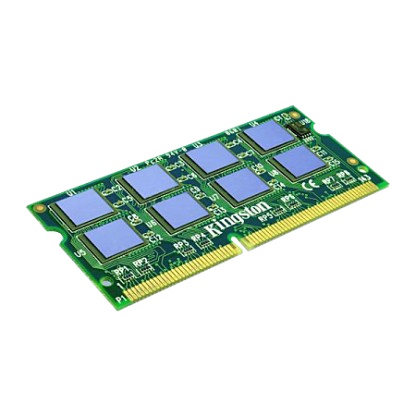
\includegraphics[scale=0.1]{images/process.png}
	  \end{figure}
	  \item Proceso
	  \begin{itemize}
	  	\item Es dinámico
	  	\item Tiene program counter
	  	\item Su ciclo de vida comprende desde que se lo ejecuta hasta que termina
	  \end{itemize}
	  \begin{figure}
			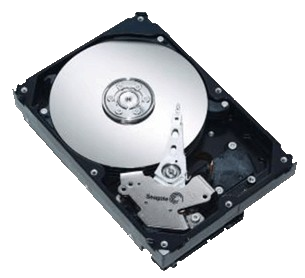
\includegraphics[scale=0.1]{images/program.png}
	  \end{figure}	  
  \end{itemize}
\end{frame}

\begin{frame}
  \frametitle{Procesos - PCB}
  \begin{itemize}
	  \item Una por proceso
	  \item Contiene información del proceso
	  \item Es lo primero que se crea cuando se realiza un \textit{fork} y lo último que se desaloca cuando termina
	  \begin{figure}
			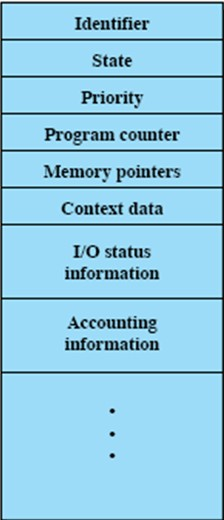
\includegraphics[scale=0.2]{images/pcb.png}
	  \end{figure}	  
  \end{itemize}
\end{frame}

\begin{frame}
  \frametitle{Procesos - Estados}
  \begin{figure}
		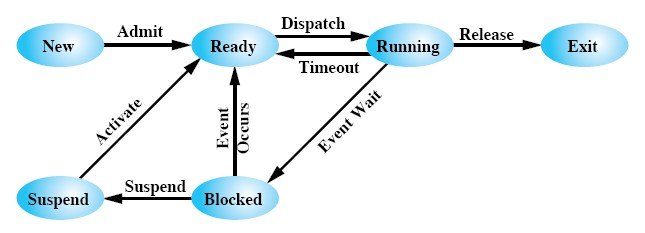
\includegraphics[scale=0.5]{images/statesProcess.png}
  \end{figure}
\end{frame}

\begin{frame}
  \frametitle{Planificadores}
  \begin{itemize}
	  \item Es la clave de la multiprogramación
	  \item Esta diseñado de manera apropiada para cumplir las metas de:
	  \begin{itemize}
	  	\item Menor Tiempo de Respuesta
	  	\item Mayor rendimiento
	  	\item Uso eficiente del procesador
	  \end{itemize}
  \end{itemize}
\end{frame}

\begin{frame}
  \frametitle{Planificadores - Tipos}
  \begin{itemize}
		\item \textit{Long term scheduler}: admite nuevos procesos a memoria (controla el grado de multirpogramación)
		\item \textit{Medium term scheduler}: realiza el \emph{swapping} (intercambio) entre el disco y la memoria cuando el SO lo determina (puede disminuir el grado de multiprogramación)
		\item \textit{Short term scheduler}: determina que proceso pasará a ejecutarse
  \end{itemize}
\end{frame}

\begin{frame}
  \frametitle{Planificadores y Estados}
  \begin{figure}
    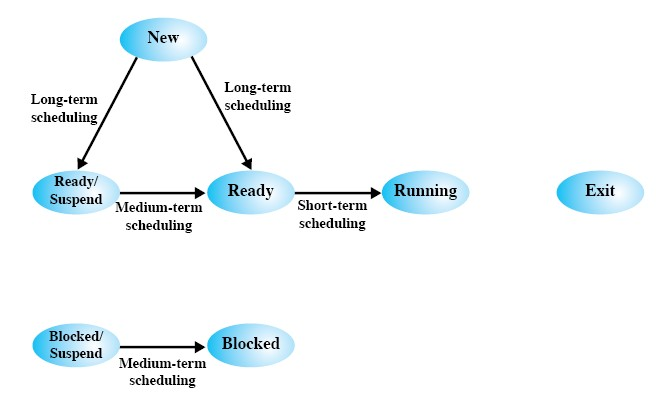
\includegraphics[scale=0.4]{images/statesSchedulers.png}
  \end{figure}
\end{frame}

\begin{frame}
  \frametitle{Planificadores y Colas}
  \begin{figure}
    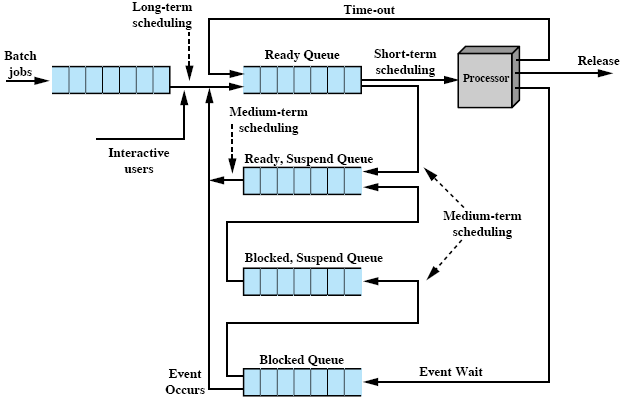
\includegraphics[scale=0.4]{images/queuesSchedulers.png}
  \end{figure}
\end{frame}

\begin{frame}
  \frametitle{Tiempos de los procesos}
  \begin{itemize}
		\item \textbf{Retorno}: tiempo que transcurre entre que el proceso llega al sistema hasta que completa su ejecución
		\item \textbf{Espera}: tiempo que el proceso se encuentra en el sistema esperando, es decir el tiempo que pasa sin ejecutarse (\textbf{TR - Tcpu})
		\item \textbf{Promedios}: tiempos promedio de los anteriores
  \end{itemize}
\end{frame}

\begin{frame}
  \frametitle{Apropiación vs No Apropiación}
  \begin{itemize}
		\item \textbf{Nonpreemptive}: una vez que un proceso esta en estado de ejecución, continua hasta que termina o se bloquea por algún evento (e.j. I/O)
		\item \textbf{Preemptive}: el proceso en ejecución puede ser interrumpido y llevado a la cola de listos:
		\begin{itemize}
			\item Mayor overhead pero mejor servicio
			\item Un proceso no monopoliza el procesador
		\end{itemize}
  \end{itemize}
\end{frame}

\begin{frame}
  \frametitle{Algoritmo \textbf{FIFO}}
  \begin{itemize}
		\item Firs come first served
		\item Cuando hay que elegir un proceso para ejecutar, se selecciona el mas viejo
		\item No favorece a ningún tipo de procesos, pero en principio prodíamos decir que los \textit{CPU Bound} terminan al comenzar su primer ráfaga, mientras que los \textit{I/O Bound} no
  \end{itemize}
\end{frame}

\begin{frame}[fragile]
  \frametitle{Algoritmo \textbf{FIFO} (cont.)}
  \begin{table}
      \centering
      \resizebox{15pc}{!}{
	  \begin{tabular}{| c | c | c | c |}
	      \hline
	      \bf Job & \bf Llegada & \bf CPU & \bf Prioridad \\
	      \hline
	      1 & 0 & 9 & 3 \\
	      \hline
	      2 & 1 & 5 & 2 \\
	      \hline
	      3 & 2 & 3 & 1 \\
	      \hline
	      4 & 3 & 7 & 2 \\
	      \hline
	  \end{tabular}
      }
  \end{table}  
  \begin{lstlisting}
#Ejemplo 1
TAREA “1” PRIORIDAD=3
[CPU,9]
TAREA “2” PRIORIDAD=2
[CPU,5]
TAREA “3” PRIORIDAD=1
[CPU,3]
TAREA “4” PRIORIDAD=2
[CPU,7]  
  \end{lstlisting}  
  \hspace{35pt} \textcolor{orange}{¿Cuáles serían los tiempos de retorno y espera?}
\end{frame}

\begin{frame}
  \frametitle{Algoritmo \textbf{SJF}}
  \begin{itemize}
  		\item Shortest Job First
		\item Política \textit{nonpreemptive} que selecciona el proceso más corto
		\item Procesos cortos se colocan delante de procesos largos
		\item Los procesos largos pueden sufrir \textit{starvation} (inanición)
  		\pause
  		\item \textcolor{orange}{Veamos el ejemplo anterior}	
  \end{itemize}
\end{frame}

\begin{frame}
  \frametitle{Algoritmo \textbf{RR}}
  \begin{itemize}
  		\item Round Robin
		\item Politica basada en un reloj
		\item \textbf{Quantum (Q)}: medida que determina cuanto tiempo podrá usar el procesador cada preceso:
		\begin{itemize}
			\item Pequeño: overhead de \textit{context switch}
			\item Grande: ¿pensar?
		\end{itemize}
		\item Cuando un proceso es expulsado de la \textit{CPU} es colocado al final de la \textit{Ready Queue} y se selecciona otro (\textit{FIFO circular})
  \end{itemize}
\end{frame}

\begin{frame}
  \frametitle{Algoritmo \textbf{RR} (cont.)}
  \begin{itemize}
  		\item Existe un ``contador'' que indica las unidades de CPU en las que el proceso se ejecuto. Cuando el mismo llega a 0 el proceso es expulsado
		\item Existen dos variantes con respecto al valor inicial del ``contador'' cuando un proceso es asignado a la CPU:
		\begin{itemize}
			\item \textbf{Timer Variable}
			\item \textbf{Timer Fijo}
		\end{itemize}
  \end{itemize}
\end{frame}

\begin{frame}
  \frametitle{Algoritmo \textbf{RR - Timer Variable}}
  \begin{itemize}
  		\item El ``contador'' se inicializa en Q (contador := Q) cada vez que un proceso es asignado a la \emph{CPU}
		\item Es el más utilizado
		\item Utilizado por el simulador
		\pause
		\item \textcolor{orange}{Veamos el ejemplo 1 nuevmanete}
  \end{itemize}
\end{frame}

\begin{frame}
  \frametitle{Algoritmo \textbf{RR - Timer Fijo}}
  \begin{itemize}
  		\item El ``contador'' se inicializa en Q cuando su valor es cero
  		\begin{itemize}
  			\item if (contador == 0) contador = Q;
  		\end{itemize}
		\item Se puede ver como un valor de Q compartido entre los procesos
  \end{itemize}
\end{frame}

\begin{frame}
  \frametitle{Algoritmo \textbf{RR} (cont.)}
	\begin{figure}
	    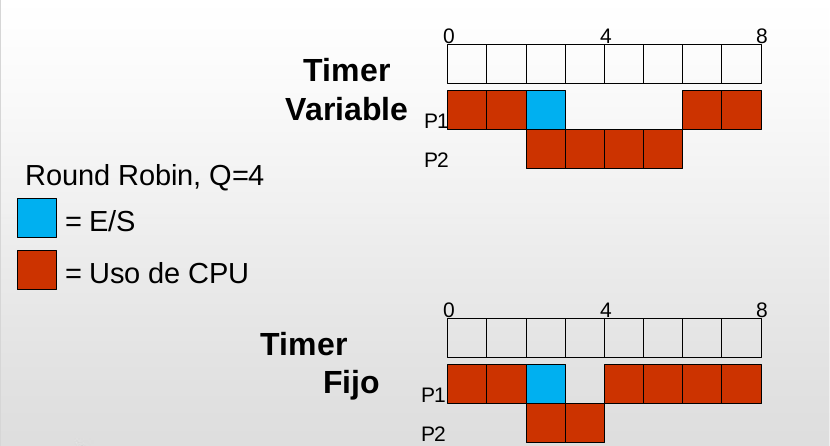
\includegraphics[scale=0.4]{images/ejemploRR.png}
	\end{figure}
\end{frame}

\begin{frame}
  \frametitle{Algoritmo con Uso de Prioridades}
  \begin{itemize}
  		\item Cada proceso tiene un valor que representa su prioridad $\rightarrow$ menor valor, mayor prioridad
		\item Se selecciona el proceso de mayor prioridad de los que se encuentran ela \emph{Ready Queue}
		\item Existe una \emph{Ready Queue} por cada nivel de prioridad
		\item Procesos de baja prioridad pueden sufrir \emph{starvation} (inanición)
		\begin{itemize}
			\item Solución: permitir a un proceso cambiar su prioridad durante su ciclo de vida $\rightarrow$ \textbf{Aging}
		\end{itemize}
		\item Es un algoritmo \textbf{preemptive}
		\pause
		\item \textcolor{orange}{Veamos el ejemplo 1 nuevamente}
  \end{itemize}
\end{frame}

\begin{frame}
  \frametitle{Algoritmo con Uso de Prioridades (cont.)}
	\begin{figure}
	    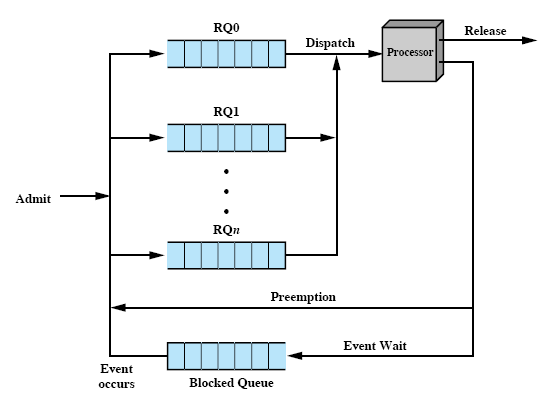
\includegraphics[scale=0.4]{images/priorities.png}
	\end{figure}
\end{frame}

\begin{frame}
  \frametitle{Algoritmo \textbf{SRTF}}
  \begin{itemize}
  		\item Shortest Remaining Time First  		
		\item Versión \emph{preemptive} de \textit{SJF}
		\item Selecciona el proceso al cual le resta menos tiempo de ejecución en su siguiente ráfaga.
		\begin{itemize}
			\item También puede ser por el tiempo dedicado a la siguiente ráfaga
		\end{itemize}
  \end{itemize}
\end{frame}

%%%%%%%%%%%%%%%%%%%%%%%%%%%%%%%%%%%%%%%%%%%%%%%%%%%%%%%%%%%%%%%%%%

\begin{comment}

\begin{frame}[fragile]
  \frametitle{Características - Configuración de discos (cont.)}
  \begin{itemize}
	  \item A futuro, todos los dispositivos llamados hdX serán denominados sdX $\leftarrow$ Introducido en Debian/Squeeze
	  \item Por estas y otras razones se adoptan 4 mecanismos nuevos para nomenclar\footnote{\url{http://wiki.debian.org/Part-UUID}}:
	  \begin{itemize}
	  	\item Nombres persistentes por \textbf{UUID} (\small{Universal Unique Identifier}):
	  	\begin{lstlisting}
$ ls –l /dev/disk/by-uuid/
2d781b26-0285-421a-b9d0-d4a0d3b55680 -> ../../sda1
31f8eb0d-612b-4805-835e-0e6d8b8c5591 -> ../../sda7
		\end{lstlisting}
		\item Utilizando \textbf{labels}
		\begin{lstlisting}
$ ls -l /dev/disk/by-label
data -> ../../sdb2
data2 -> ../../sda2
		\end{lstlisting}
	  \end{itemize}
  \end{itemize}
\end{frame}

\begin{frame}
  \frametitle{Herramientas para particionar}
  \begin{itemize}
	  \item El particionado de un disco se lo puede realizar mediante:
	  \begin{itemize}
	  	\item Software destructivo: \textit{fdisk}
	  	\item Software no destructivo: \textit{fips}, \textit{gparted}
		\begin{figure}
		    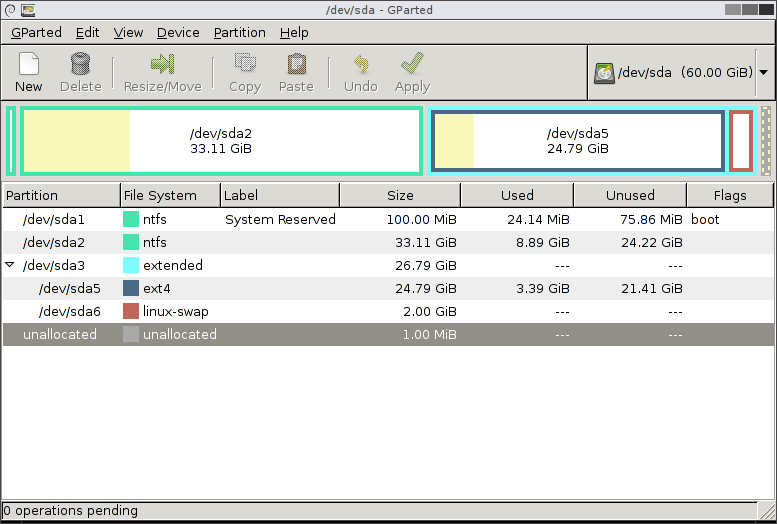
\includegraphics[scale=0.3]{images/gparted.png}
		\end{figure}
	  \end{itemize}
  \end{itemize}
\end{frame}

\begin{frame}[fragile]
  \frametitle{Permisos}
  \begin{itemize}
	  	\item Se aplican a directorios y archivos
	  	\item Existen 3 tipos de permisos y se basan en una notación octal:
	  	\begin{table}
		      \centering
		      \resizebox{10pc}{!}{
			  \begin{tabular}{| c | c | c |}
			      \hline
			      \bf Permiso & \bf Valor & \bf Octal \\
			      \hline
			      Lectura & R & 4 \\
			      \hline
			      Escritura & W & 2 \\
			      \hline
			      Ejecución & X & 1 \\
			      \hline
			  \end{tabular}
		      }
		\end{table}
		\item Se aplican sobre los usuarios:
		\begin{itemize}
			\item Usuario: permisos del dueño $\rightarrow$ \textbf{U}
			\item Usuario: permisos del grupo $\rightarrow$ \textbf{G}
			\item Usuario: permisos de otros usuario $\rightarrow$ \textbf{O}
		\end{itemize}
		\item Se utiliza el comando \textbf{chmod}:
		\begin{lstlisting}
$ chmod 755 /tmp/script
		\end{lstlisting}
  \end{itemize}
\end{frame}
\end{comment}